\chapter{Air Separation Technology}
\label{chp:airsep}
\begin{figure}[h]
	\begingroup%
  \makeatletter%
    \setlength{\unitlength}{1cm}%
  \makeatother%
  \begin{picture}(17, 7)%	
    \scriptsize
    \put(2,1){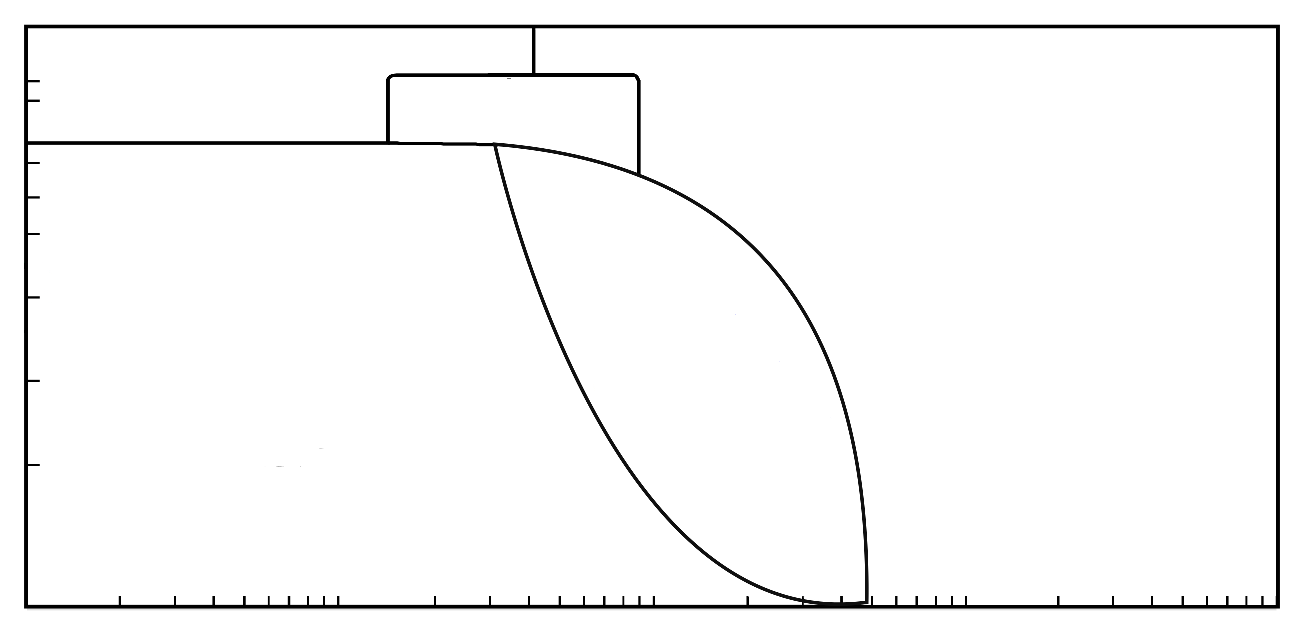
\includegraphics[width=13cm]{Pictures/tech_comp_graph.eps}}%
    \put(8.5, 0.1){\color[rgb]{0,0,0}\makebox(0,0)[c]{\smash{\normalsize{product stream $[\frac{m^3_{STP}}{h}]$}}}}%
    \put(0.6, 4){\color[rgb]{0,0,0}\rotatebox{90}{\makebox(0,0)[c]{\smash{\normalsize{$N_2$-purity $x_{N_2, Ret}$ $[\%]$}}}}}%
    \put(1.9, 0.65){\color[rgb]{0,0,0}\makebox(0,0)[l]{\smash{$10$}}}%
    \put(5.15, 0.65){\color[rgb]{0,0,0}\makebox(0,0)[l]{\smash{$10^2$}}}%
    \put(8.35, 0.65){\color[rgb]{0,0,0}\makebox(0,0)[l]{\smash{$10^3$}}}%
    \put(11.55, 0.65){\color[rgb]{0,0,0}\makebox(0,0)[l]{\smash{$10^4$}}}%
    \put(14.75, 0.65){\color[rgb]{0,0,0}\makebox(0,0)[l]{\smash{$10^5$}}}%
    \put(1.85, 1){\color[rgb]{0,0,0}\makebox(0,0)[r]{\smash{$95$}}}%
    \put(1.85, 2.45){\color[rgb]{0,0,0}\makebox(0,0)[r]{\smash{$97$}}}%
    \put(1.85, 3.325){\color[rgb]{0,0,0}\makebox(0,0)[r]{\smash{$98$}}}%
    \put(1.85, 4.15){\color[rgb]{0,0,0}\makebox(0,0)[r]{\smash{$99$}}}%
    \put(1.85, 4.8){\color[rgb]{0,0,0}\makebox(0,0)[r]{\smash{$99.5$}}}%
    \put(1.85, 5.2){\color[rgb]{0,0,0}\makebox(0,0)[r]{\smash{$99.9$}}}%
    \put(1.85, 5.55){\color[rgb]{0,0,0}\makebox(0,0)[r]{\smash{$99.95$}}}%
    \put(1.85, 6.1){\color[rgb]{0,0,0}\makebox(0,0)[r]{\smash{$99.99$}}}%
    \put(1.85, 6.4){\color[rgb]{0,0,0}\makebox(0,0)[r]{\smash{$99.999$}}}%
    \put(1.85, 6.4){\color[rgb]{0,0,0}\makebox(0,0)[r]{\smash{}}}%
    \put(5,3){\color[rgb]{0,0,0}\normalsize{\CM{membrane processes / \\ gas permeation}}}%
    \put(8.9,3.7){\color[rgb]{0,0,0}\normalsize{\CM{PSA}}}%
    \put(7,6.20){\color[rgb]{0,0,0}\scriptsize{\CM{membrane \& \\ post oxidation}}}%
    \put(4,6.5){\color[rgb]{0,0,0}\normalsize{\CM{cryogenic processes \\ (liquid)}}}%
    \put(12,5.5){\color[rgb]{0,0,0}\normalsize{\CM{cryogenic processes \\ (gaseous)}}}%
  \end{picture}%
\endgroup%

	\caption{Comparison of Air Separation Technologies \cite{Prasad.1994}.}
	\label{fig:tech_compar}
\end{figure}

There are several ways besides cryogenic air separation that can be employed to separate gas mixtures. 
In this chapter different competing technologies and their main applications will be discussed. The 
predominately used technologies are cryogenic distillation, pressure swing adsorption (PSA) as well as 
gas permeation (GP). In the distillation process the gas is first liquefied. Separation is the achieved 
by the different concentration differences in vapor and liquid phase. PSA relies on the different affinities 
of gaseous species to adsorb to certain materials in order to extract a component form a mixture. During gas 
permeation membranes are used. Each species migrates in different quantities through a given membrane
depending on process parameters and membrane structure. 

\reffig{fig:tech_compar} illustrates the most economically viable processes depending on product
purity and product stream volume. It can be seen that alternative air separation processes 
cannot supply the high quality or quantity of the cryogenic process. Due to that cryogenic air separation is 
thought to be the main supplier of highly pure gases in industrial quantities for years to come \cite{Zhu.2010}. 
The alternative processes however offer some very appealing characteristics, which make them the 
favorable choice when lower quantities of product or more moderate purity is required. The cryogenic 
process is always connected with an considerable energy consumption for the liquefaction and compression. 
Due to that smaller implementations of the process a very unlikely to yield economically sound solutions
to a separation problem. 

\addref

\section{Cryogenic Air Separation}
\label{sec:cryo_air_sep}

\section{Pressure Swing Adsorbtion}
\label{sec:psa}

\section{Gas Permeation}
\label{sec:membrane}
\todo[inline]{find paper: DOI: 10.1002/cite.330480804}
The separation of mixed gases by membrane process is called gas permeation. Its main strength 
in comparison with alternative processes are the low energy consumption and the possibility to 
produce flexible mobile units. As mentioned before it is not however capable of producing high
quantity highly pure product streams. As \reffig{fig:tech_compar} illustrates the main application 
for the gas permeation process are small to moderate product streams at intermediate purities.   

\begin{figure}
	\center
	
\begingroup%
  \makeatletter%
    \setlength{\unitlength}{1cm}%
  \makeatother%
  \begin{picture}(13, 7)%	
    \put(0,0){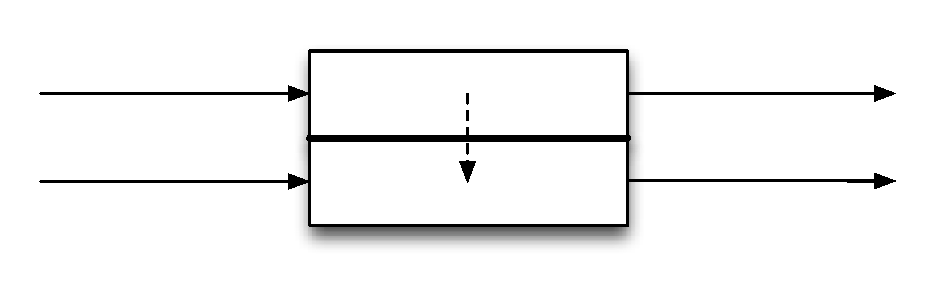
\includegraphics[width=13cm]{Pictures/gas_permeation.eps}}%
    \put(2.3, 1.5){\color[rgb]{0,0,0}\makebox(0,0)[c]{\smash{sweep}}}%
     \put(2.3, 2.8){\color[rgb]{0,0,0}\makebox(0,0)[c]{\smash{feed}}}%
     \put(10.7, 1.5){\color[rgb]{0,0,0}\makebox(0,0)[c]{\smash{retentate}}}%
     \put(10.7, 2.8){\color[rgb]{0,0,0}\makebox(0,0)[c]{\smash{permeate}}}%
  \end{picture}%
\endgroup%

	\caption{Gas permeation process.}
	\label{fig:gas_permeation} 
\end{figure}

\reffig{fig:gas_permeation} shows the schematic for a single stage membrane unit. Within the feed stream 
the gaseous mixture is fed into the unit, which can quickly be implemented. Within the unit one or more 
species migrate favorably through the membrane. In this case mostly dense polymer membranes are 
employed used. There have been some impressive results with metallic membranes, but due to 
the very high material costs they have not been adapted by the industry. Furthermore, since gaseous 
phases often have rather small molecular species, porous membranes cannot achieve desired separation. 
The driving force the separation process is a difference in partial pressure or species activity across the 
membrane. According to the molecular structure of each species, the structure of the separating membrane 
as well as the process parameters pressure and temperature, they permeate through the membrane in 
different quantities.

The process of permeation can be subdivided into three separate steps. Sorption at the membrane / 
feed interface, diffusion through the mostly dense polymer membrane and finally desorption at the 
permeate side of the membrane. 
